% The default theme, with plain white background
%\documentclass[bgimages]{smilebeamer}

% If you don't like oranges and such in the background remove the [bgimages] like this :
\documentclass{smilebeamer}

\usepackage[francais]{babel}
\usepackage[utf8]{inputenc}
\usepackage{eurosym}
\usepackage{hyperref}
\usepackage{minted}

\title{Bluetooth Low Energy}
\author{maxime.chevallier@smile.fr}

\begin{document}

%%%%%%%%%%%%%%%%%%%%%%%%%%%%%
\begin{frame}[plain]
    \title{Bluetooth Low Energy}
    \subtitle{Présentation et Utilisation sous Linux}
    \titlepage
\end{frame}


\section{Bluetooth}

\begin{frame}[t]
	\frametitle{Bluetooth}

	\begin{minipage}[t]{0.50\linewidth}
		\begin{block}{Historique}
			\begin{itemize}
				\item 1994 : Création
				\item 1998 : SIG
				\item 1999 : 1.0
				\item 2004 : 2.0 BR / EDR
				\item 2010 : 4.0 BLE
				\item 2014 : 4.2
			\end{itemize}
		\end{block}
	\end{minipage}
	\begin{minipage}[t]{0.25\linewidth}
		\begin{figure}
			
\includegraphics[height=2.5cm]{img/bt_logo.png}
		\end{figure}
	\end{minipage}
\end{frame}

\begin{frame}
	\frametitle{Standard Bluetooth}
	\center{\textbf{Services}, \textbf{Profils} et \textbf{Protocoles}}
	\vspace{0.5cm}
	\begin{itemize}
		\item Liaison physique
		\item Adressage physique
		\item Controle de flux
		\item Multiplexage
		\item Chiffrement
		\item Protocoles over Bluetooth
		\item "Profils"
	\end{itemize}
	\vspace{0.5cm}
	\tiny{\url{https://www.bluetooth.com/specifications/adopted-specifications}}
\end{frame}

\begin{frame}
	\frametitle{Dénomination}

	\begin{minipage}[t]{0.30\linewidth}
		\begin{block}{Classique}
			\begin{itemize}
				\item Classique
				\item BR/EDR
				\item 2.0 3.0 3.1
				\item Bluetooth
			\end{itemize}
		\end{block}
		\begin{figure}
			
\includegraphics[width=\linewidth]{img/Bluetooth_Logo.png}
		\end{figure}
	\end{minipage}
	\begin{minipage}[t]{0.30\linewidth}
		\begin{block}{Les deux}
			\begin{itemize}
				\item Dual mode
				\item Smart Ready
				\item 4.0 4.1 4.2
			\end{itemize}
		\end{block}
		\begin{figure}
			
\includegraphics[width=\linewidth]{img/Bluetooth_Smart_Ready_Logo.jpg}
		\end{figure}
	\end{minipage}
	\begin{minipage}[t]{0.30\linewidth}
		\begin{block}{Low Energy}
			\begin{itemize}
				\item Low Energy
				\item Smart
				\item Wibree
				\item 4.0 4.1 4.2
			\end{itemize}
		\end{block}
		\begin{figure}
			
\includegraphics[width=\linewidth]{img/Bluetooth_Smart_Logo.png}
		\end{figure}
	\end{minipage}
\end{frame}


\begin{frame}
	\frametitle{Architecture physique}
	\begin{block}{Host et controller séparés}
		\begin{minipage}[t]{0.48\linewidth}
		\begin{figure}
			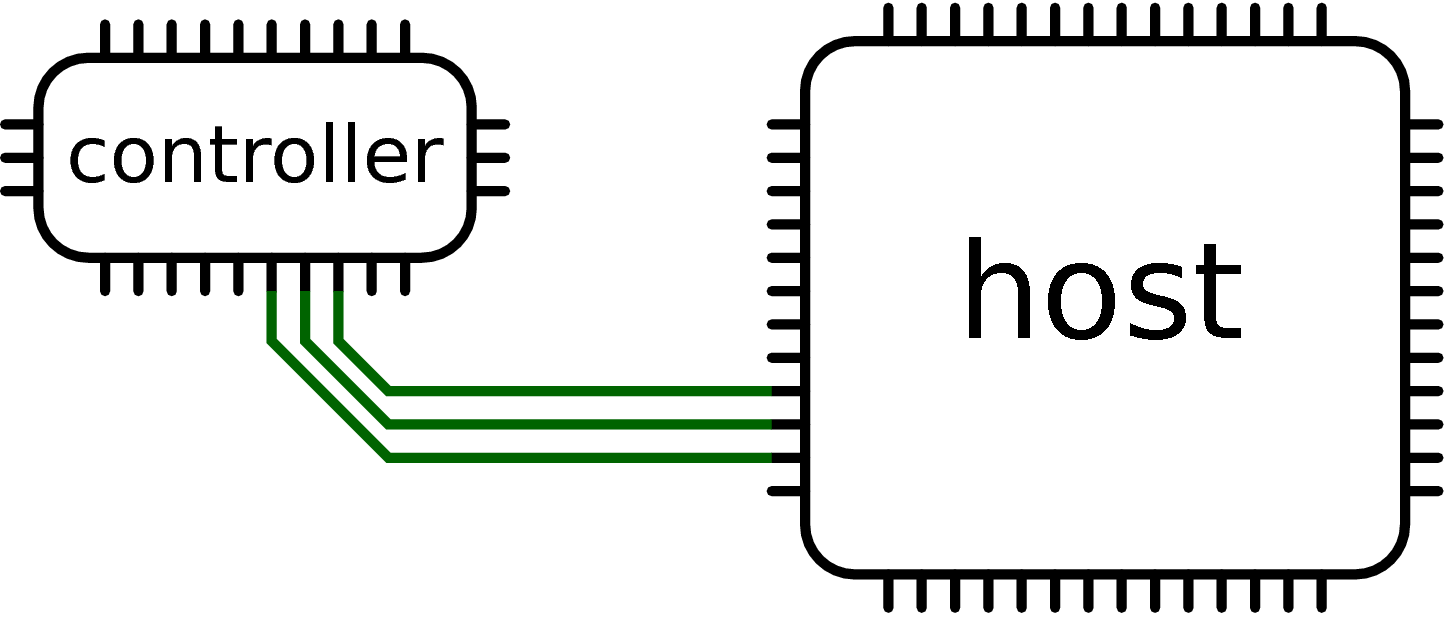
\includegraphics[width=4cm]{img/HC_sep.png}
		\end{figure}
		\end{minipage}
		\begin{minipage}[t]{0.48\linewidth}
		\begin{figure}
			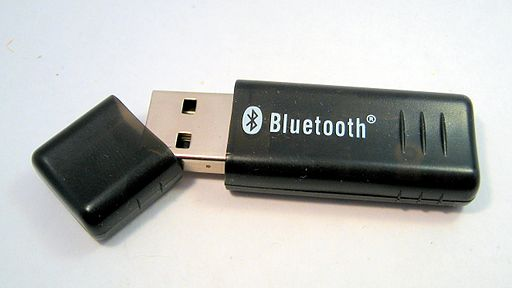
\includegraphics[width=3cm]{img/dongle.jpg}
		\end{figure}
		\end{minipage}
	\end{block}
	\begin{block}{System on a Chip}
		\begin{minipage}[t]{0.48\linewidth}
		\begin{figure}
			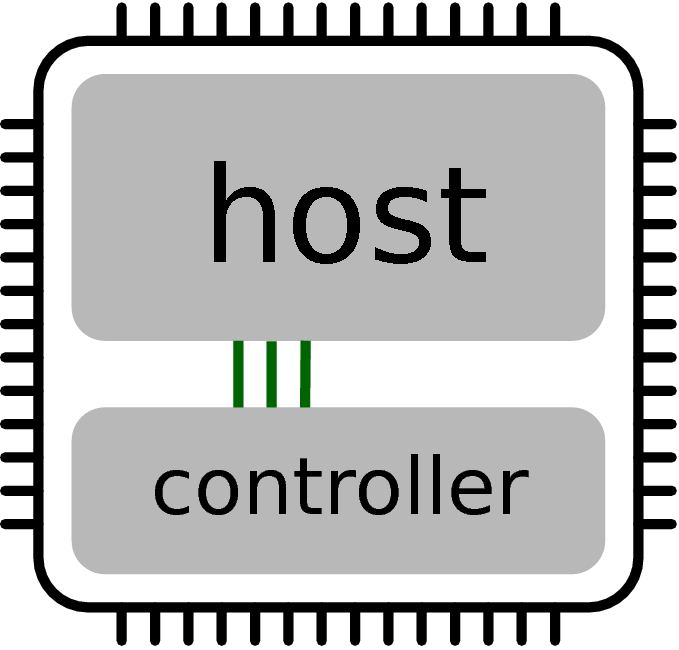
\includegraphics[width=2cm]{img/HC_soc.png}
		\end{figure}
		\end{minipage}
		\begin{minipage}[t]{0.48\linewidth}
		\begin{figure}
			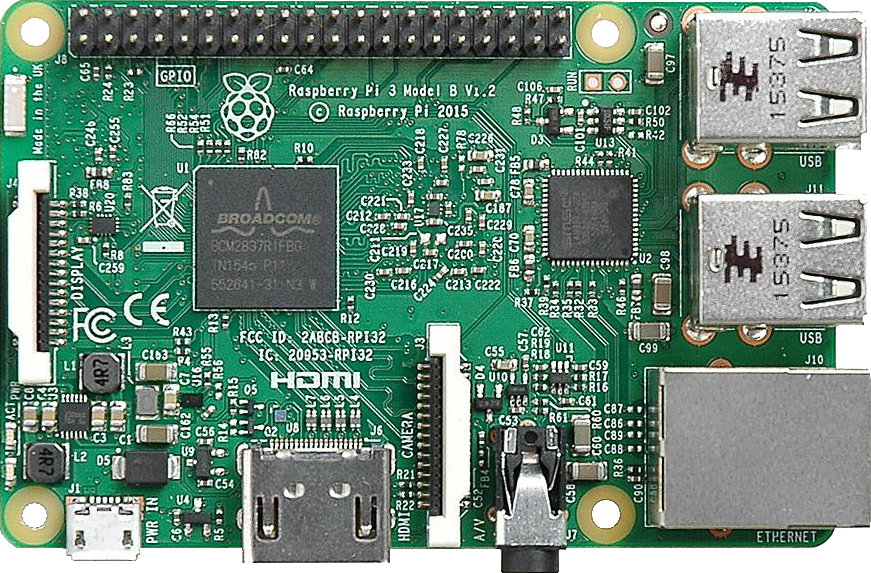
\includegraphics[width=3cm]{img/rpi3.png}
		\end{figure}
		\end{minipage}
	\end{block}
\end{frame}


\begin{frame}[t]
	\frametitle{Bluetooth Classique}
	\begin{minipage}[t]{0.30\linewidth}
		\vspace{0.5cm}
		\begin{block}{Radio}
			\begin{itemize}
				\item 2.4 GHZ
				\item 79 canaux
				\item FHSS
			\end{itemize}
		\end{block}
	\end{minipage}
	\begin{minipage}[t]{0.66\linewidth}
		\vspace{0.5cm}
		\center{\Large{Profils}}
		\vspace{0.5cm}
		\begin{itemize}
			\item Audio
			\item Transfert de fichiers
			\item IP / LAN
			\item Port série
			\item Partage de contacts
			\item Human Interface Device
			\item Découverte de services
		\end{itemize}
	\end{minipage}
\end{frame}

\begin{frame}
	\frametitle{Architecture logique}
	\begin{minipage}{0.45\linewidth}
		\begin{figure}
			\includegraphics[height=6cm]{img/HCI.png}
		\end{figure}
	\end{minipage}
	\begin{minipage}{0.50\linewidth}
		\begin{block}{Host}
			\begin{itemize}
				\item Profils et applications
				\item Différents protocoles
				\item Abstraction
				\item Multiplexage
			\end{itemize}
		\end{block}
		\begin{block}{Controller}
			\begin{itemize}
				\item Chiffrement
				\item Connexion
				\item Transmission physique
			\end{itemize}
		\end{block}
	\end{minipage}
\end{frame}


\section{Bluetooth Low Energy}

\begin{frame}
	\frametitle{Bluetooth Low Energy}
	\begin{minipage}[t]{0.30\linewidth}
		\vspace{0.5cm}
		\begin{block}{Radio}
			\begin{itemize}
				\item 2.4 GHZ
				\item 40 canaux
			\end{itemize}
		\end{block}
	\end{minipage}
	\begin{minipage}[t]{0.66\linewidth}
		\vspace{0.5cm}
		\center{\Large{Services}}
		\vspace{0.5cm}
		\begin{itemize}
			\item "Healthcare"
			\item "Fitness"
			\item "Human Interface Device"
			\item "Alert"
			\item "Proximity"
			\item Capteurs génériques
			\item Découverte de services
			\item Et bien plus...
		\end{itemize}
	\end{minipage}
\end{frame}

\begin{frame}
	\frametitle{Stack BLE}
	\begin{minipage}{0.45\linewidth}
		\begin{figure}
			\includegraphics[height=6cm]{img/HCI_GATT.png}
		\end{figure}
	\end{minipage}
	\begin{minipage}{0.50\linewidth}
		\begin{block}{Stack Bluetooth Low Energy}
			\begin{itemize}
				\item Link Layer
				\item L2CAP
				\item Protocole ATT
				\item Profile GATT
				\item Services : Application
			\end{itemize}
		\end{block}
	\end{minipage}
\end{frame}

\begin{frame}
	\frametitle{Link Layer}
	\begin{minipage}{0.60\linewidth}
		\begin{figure}
			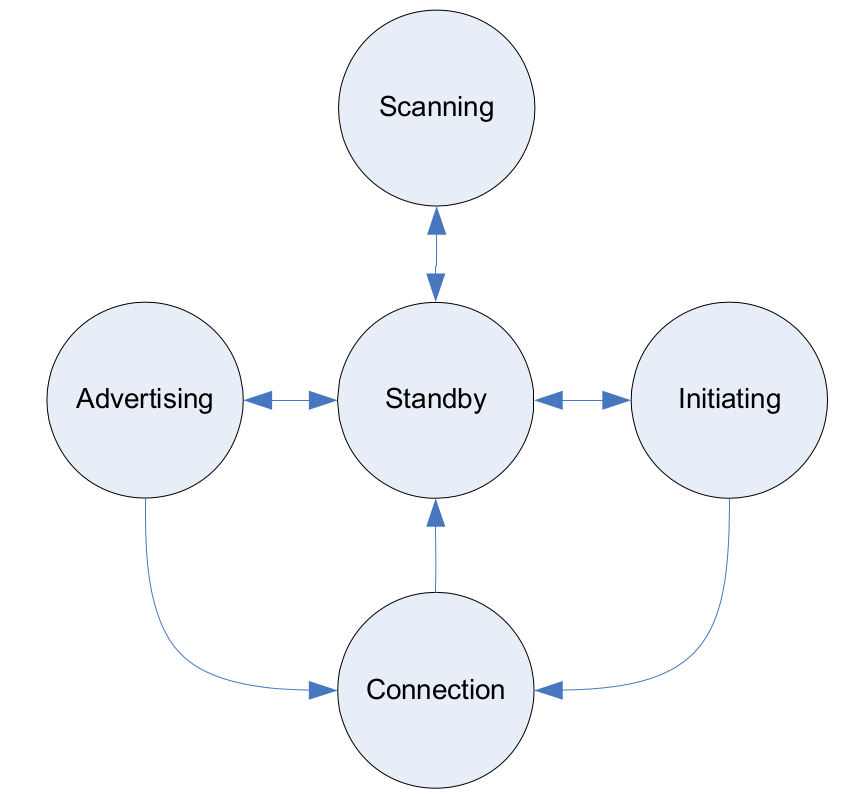
\includegraphics[height=6cm]{img/BLE_LL.png}
		\end{figure}
	\end{minipage}
	\begin{minipage}{0.35\linewidth}
		\begin{itemize}
			\item Idle \\ {\tiny{On ne fait rien}}
			\item Advertising \\ {\tiny{Broadcast, connectable ou non}}
			\item Scanning \\ {\tiny{Ecoute d'advertisements}}
			\item Initiating \\ {\tiny{Ecoute d'advertisements}} \\
								{\tiny{Réponse par connexion}}
			\item Connection \\ {\tiny{Connecté}} \\
				{\tiny{Master (depuis Initiating) ou}} \\
				{\tiny{Slave (Depuis Advertising)}}
		\end{itemize}
	\end{minipage}
\end{frame}



\section{Les choses se GATT}

\begin{frame}
	\center{\huge{ATT}}
\end{frame}

\begin{frame}
	\center{\huge{GATT}}
\end{frame}

\begin{frame}
	\center{\huge{Exemple de service}}
\end{frame}

\section{BLE dans Linux}

\begin{frame}
	\frametitle{BlueZ}
	\begin{block}{Historique}
		\begin{itemize}
			\item 2001 : Max Krasnyansky ( Qualcomm ) {\small{\textit{linux 2.4.6}}}
			\item 2004 : Marcel Holtmann ( Intel ) {\small{\textit{linux 2.6}}}
			\item 2012 : Low Energy ( BlueZ 5.0 ) {\small{\textit{linux 3.5}}}
			\item 2016 : BlueZ 5.43
		\end{itemize}
	\end{block}

	\vspace{1cm}
	\textbf{APIs} : \textit{DBus}, \textit{Socket}, \textit{Librairie C}
\end{frame}

\begin{frame}
	\frametitle{Bluez : Architecture}
	\begin{minipage}{0.50\linewidth}
	\begin{figure}
		\includegraphics[height=5cm]{img/bluez.png}
	\end{figure}
	\end{minipage}
	\begin{minipage}{0.32\linewidth}
		\begin{block}{userspace}
			\begin{itemize}
				\item Profils
				\item API Dbus
				\item Bluetoothd \\ {\tiny{le démon à tout faire}}
			\end{itemize}
		\end{block}
		\begin{block}{kernel}
			\begin{itemize}
				\item HCI
				\item Drivers
				\item Protocoles
				\item mgmt \\ {\small{l'API à tout faire}}
			\end{itemize}
		\end{block}
	\end{minipage}
\end{frame}

\begin{frame}
	\frametitle{Outils pratiques}
	\begin{minipage}{0.46\linewidth}
		\begin{block}{bluetoothctl}
			\begin{itemize}
				\item UI de bluetoothd
				\item Gestion des appareils
				\item Gestion des profils
			\end{itemize}
		\end{block}
		\begin{block}{btmon}
			\begin{itemize}
				\item Monitore HCI
				\item Monitore MGMT
				\item Excellent pour le debug
			\end{itemize}
		\end{block}
	\end{minipage}
	\begin{minipage}{0.46\linewidth}
		\begin{block}{btmgmt}
			\begin{itemize}
				\item Utilise la MGMT API
				\item Gestion du controller
				\item Gestion du dual-mode
			\end{itemize}
		\end{block}
		\begin{block}{GATT}
			\begin{itemize}
				\item gatttool
				\item btgatt-client
				\item btgatt-server
			\end{itemize}
		\end{block}
	\end{minipage}
	\vspace{0.5cm}
	\small{

	\textbf{A voir aussi} : \textit{obexctl}, \textit{rfcomm}, \textit{l2ping}, \textit{hciattach}

	\textbf{Déprécié} : \textit{hciconfig}, \textit{hcitool}, \textit{hcidump}, \textit{sdptool}
	}

\end{frame}


\begin{frame}
	\frametitle{Démo}

	\vspace{1cm}
	\textbf{Laptop} : {\small{\textit{Intel 7265, linux 3.19, BlueZ 5.37}}}
	
	{\small{Host - Controller : PCI}}

	\vspace{1cm}
	\textbf{TI Sensortag} :{\small{\textit{TI CC2650, Démonstrateur BLE avec capteurs embarqués, OS TI}}}
	
	{\small{Host - Controller : SoC}}

	\vspace{1cm}
	\textbf{Wistiki} : {\small{\textit{nRF8002, "Tag" connecté, profils "Alert" et "Proximity"}}}
	
	{\small{Host - Controller fusionnés, pas de HCI}}
\end{frame}

\begin{frame}
	\frametitle{C'est fini}
	\center{\huge{Merci}}
\end{frame}
\end{document}

